\documentclass[../main]{subfiles}

\questiontrue
\solutiontrue

\begin{document}
    \ifquestion
    
    \section{The Conics of Narnia}
	
	Aslan planned to create a new universe in such a way that this time there would be no interference from evil, as there was with Narnia. At a certain moment during its creation, while designing gravitation, he defined that the attraction between two bodies would be given by the relation: \( \vec{F} = -\frac{GMm}{d^2} \hat{d} \). Thus, help Aslan and prove some properties of the orbits of a mass \( m \) around a mass \( M \) with \( (m \ll M) \):  

Define: \( m(x,y) \) as the position of \( m \) in the orbital plane, and analogously, \( M(0,0) \) as the position of \( M \) in the orbital plane. In this case, we consider \( M \) as the origin.  

\ut{a} Given that the velocity of \( m \), at a distance \( d \) from \( M \), follows the relation:  

\[
v^2 < \frac{2GM}{d}
\]

Consider a circumference \( \Omega(x_j,y_j) \) centered at \( m(x_j,y_j) \) and passing through \( M(0,0) \). Define (at first without physical meaning) the orbit space as all points belonging to a given circumference \( \Omega(x_i,y_i) \). Prove that the orbit space is a filled circle of radius \( R = \frac{2GMd}{2GM - v^2 d} \) centered at the other focus of the orbit (the focus different from \( M(0,0) \)).  

\ut{b} Given that the velocity of \( m \), at a distance \( d \) from \( M \), follows the relation:  

\[
v^2 = \frac{2GM}{d}
\]

Show that there exists a line \( r \) in the orbital plane such that the distance between \( m(x_i,y_i) \) and \( M(0,0) \) is equal to the distance between \( m(x_i,y_i) \) and its orthogonal projection onto \( r \).  

\ut{c} What must be the velocity relation so that the region that does not belong to the orbit space (as defined in item \textbf{a)}) is a circumference centered at the other focus of the orbit (the focus different from \( M(0,0) \))?
	
	\clearpage
    
    
    \fi
    
    \ifsolution
    
    \section{The Conics of Narnia}

\ut{a} Note that the gravitational law is the same as in our universe, so all physical principles remain the same. Since \( v^2 < \frac{2GM}{d} \), we know that this is a closed orbit (velocity lower than the escape velocity), meaning it is an ellipse, as shown in Figure \ref{fig:orbitelipsi1} ("B" represents the other focus of the orbit).
	
	\begin{figure}[htpb]
	    \centering
	    

\tikzset{every picture/.style={line width=0.75pt}} %set default line width to 0.75pt        

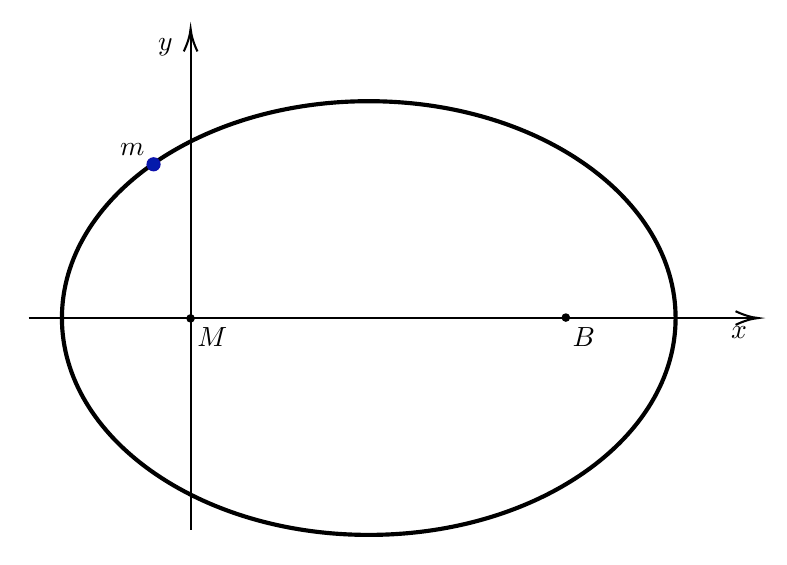
\begin{tikzpicture}[x=0.75pt,y=0.75pt,yscale=-1,xscale=1]
%uncomment if require: \path (0,542); %set diagram left start at 0, and has height of 542

%Shape: Ellipse [id:dp8979721006541848] 
\draw  [color={rgb, 255:red, 0; green, 0; blue, 0 }  ,draw opacity=1 ][line width=1.5]  (148.5,146.82) .. controls (148.5,89.12) and (214.69,42.34) .. (296.33,42.34) .. controls (377.98,42.34) and (444.17,89.12) .. (444.17,146.82) .. controls (444.17,204.52) and (377.98,251.3) .. (296.33,251.3) .. controls (214.69,251.3) and (148.5,204.52) .. (148.5,146.82) -- cycle ;
%Straight Lines [id:da5987369599518098] 
\draw [color={rgb, 255:red, 0; green, 0; blue, 0 }  ,draw opacity=1 ][line width=0.75]    (132.5,146.82) -- (482,146.82) ;
\draw [shift={(484,146.82)}, rotate = 180] [color={rgb, 255:red, 0; green, 0; blue, 0 }  ,draw opacity=1 ][line width=0.75]    (10.93,-3.29) .. controls (6.95,-1.4) and (3.31,-0.3) .. (0,0) .. controls (3.31,0.3) and (6.95,1.4) .. (10.93,3.29)   ;
%Straight Lines [id:da304235614337492] 
\draw [color={rgb, 255:red, 0; green, 0; blue, 0 }  ,draw opacity=1 ][line width=0.75]    (210.5,248.92) -- (210.5,9.42) ;
\draw [shift={(210.5,7.42)}, rotate = 90] [color={rgb, 255:red, 0; green, 0; blue, 0 }  ,draw opacity=1 ][line width=0.75]    (10.93,-3.29) .. controls (6.95,-1.4) and (3.31,-0.3) .. (0,0) .. controls (3.31,0.3) and (6.95,1.4) .. (10.93,3.29)   ;
%Shape: Circle [id:dp3527055407446611] 
\draw  [fill={rgb, 255:red, 0; green, 0; blue, 0 }  ,fill opacity=1 ] (208.7,146.99) .. controls (208.7,146) and (209.5,145.2) .. (210.49,145.2) .. controls (211.47,145.2) and (212.27,146) .. (212.27,146.99) .. controls (212.27,147.97) and (211.47,148.77) .. (210.49,148.77) .. controls (209.5,148.77) and (208.7,147.97) .. (208.7,146.99) -- cycle ;
%Shape: Circle [id:dp8770097356475901] 
\draw  [fill={rgb, 255:red, 0; green, 0; blue, 0 }  ,fill opacity=1 ] (389.5,146.59) .. controls (389.5,145.6) and (390.3,144.8) .. (391.29,144.8) .. controls (392.27,144.8) and (393.07,145.6) .. (393.07,146.59) .. controls (393.07,147.57) and (392.27,148.37) .. (391.29,148.37) .. controls (390.3,148.37) and (389.5,147.57) .. (389.5,146.59) -- cycle ;
%Shape: Circle [id:dp5217054691233125] 
\draw  [color={rgb, 255:red, 14; green, 16; blue, 171 }  ,draw opacity=1 ][fill={rgb, 255:red, 4; green, 26; blue, 171 }  ,fill opacity=1 ] (189.5,72.75) .. controls (189.5,71.01) and (190.91,69.6) .. (192.65,69.6) .. controls (194.39,69.6) and (195.8,71.01) .. (195.8,72.75) .. controls (195.8,74.49) and (194.39,75.9) .. (192.65,75.9) .. controls (190.91,75.9) and (189.5,74.49) .. (189.5,72.75) -- cycle ;

% Text Node
\draw (189.5,70) node [anchor=south east][inner sep=0.75pt]    {$m$};
% Text Node
\draw (212.49,150.39) node [anchor=north west][inner sep=0.75pt]    {$M$};
% Text Node
\draw (393.29,149.99) node [anchor=north west][inner sep=0.75pt]    {$B$};
% Text Node
\draw (193.6,10.96) node [anchor=north west][inner sep=0.75pt]    {$y$};
% Text Node
\draw (469.6,149.8) node [anchor=north west][inner sep=0.75pt]    {$x$};


\end{tikzpicture}
	    \caption{Scheme of an elliptical orbit, from point $m$, from foci $M$ and $B$}
	    \label{fig:orbitelipsi1}
	\end{figure}
	

	Now, tracing the circle $\Omega$ with center at "$m$" and passing through "$M$" we will have the representation of the figure \ref{fig:orbitelipsi2}:
	
	
	\begin{figure}[htpb]
	    \centering
	    

\tikzset{every picture/.style={line width=0.75pt}} %set default line width to 0.75pt        

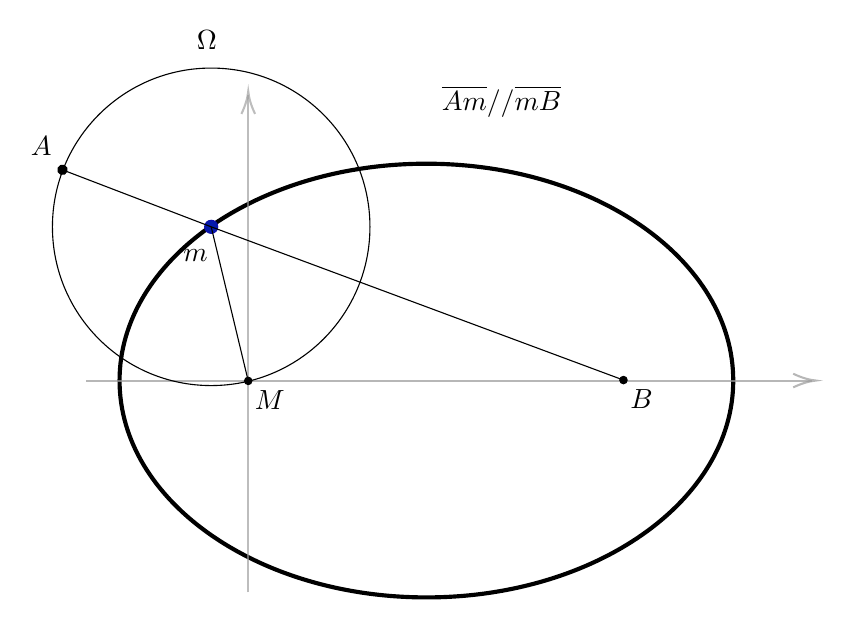
\begin{tikzpicture}[x=0.75pt,y=0.75pt,yscale=-1,xscale=1]
%uncomment if require: \path (0,542); %set diagram left start at 0, and has height of 542

%Shape: Ellipse [id:dp8979721006541848] 
\draw  [color={rgb, 255:red, 0; green, 0; blue, 0 }  ,draw opacity=1 ][line width=1.5]  (148,234.32) .. controls (148,176.62) and (214.19,129.84) .. (295.83,129.84) .. controls (377.48,129.84) and (443.67,176.62) .. (443.67,234.32) .. controls (443.67,292.02) and (377.48,338.8) .. (295.83,338.8) .. controls (214.19,338.8) and (148,292.02) .. (148,234.32) -- cycle ;
%Straight Lines [id:da5987369599518098] 
\draw [color={rgb, 255:red, 155; green, 155; blue, 155 }  ,draw opacity=0.72 ][line width=0.75]    (132,234.32) -- (481.5,234.32) ;
\draw [shift={(483.5,234.32)}, rotate = 180] [color={rgb, 255:red, 155; green, 155; blue, 155 }  ,draw opacity=0.72 ][line width=0.75]    (10.93,-3.29) .. controls (6.95,-1.4) and (3.31,-0.3) .. (0,0) .. controls (3.31,0.3) and (6.95,1.4) .. (10.93,3.29)   ;
%Straight Lines [id:da304235614337492] 
\draw [color={rgb, 255:red, 155; green, 155; blue, 155 }  ,draw opacity=0.66 ][line width=0.75]    (210,336.42) -- (210,96.92) ;
\draw [shift={(210,94.92)}, rotate = 90] [color={rgb, 255:red, 155; green, 155; blue, 155 }  ,draw opacity=0.66 ][line width=0.75]    (10.93,-3.29) .. controls (6.95,-1.4) and (3.31,-0.3) .. (0,0) .. controls (3.31,0.3) and (6.95,1.4) .. (10.93,3.29)   ;
%Shape: Circle [id:dp3527055407446611] 
\draw  [fill={rgb, 255:red, 0; green, 0; blue, 0 }  ,fill opacity=1 ] (208.2,234.49) .. controls (208.2,233.5) and (209,232.7) .. (209.99,232.7) .. controls (210.97,232.7) and (211.77,233.5) .. (211.77,234.49) .. controls (211.77,235.47) and (210.97,236.27) .. (209.99,236.27) .. controls (209,236.27) and (208.2,235.47) .. (208.2,234.49) -- cycle ;
%Shape: Circle [id:dp8770097356475901] 
\draw  [fill={rgb, 255:red, 0; green, 0; blue, 0 }  ,fill opacity=1 ] (389,234.09) .. controls (389,233.1) and (389.8,232.3) .. (390.79,232.3) .. controls (391.77,232.3) and (392.57,233.1) .. (392.57,234.09) .. controls (392.57,235.07) and (391.77,235.87) .. (390.79,235.87) .. controls (389.8,235.87) and (389,235.07) .. (389,234.09) -- cycle ;
%Shape: Circle [id:dp5217054691233125] 
\draw  [color={rgb, 255:red, 14; green, 16; blue, 171 }  ,draw opacity=1 ][fill={rgb, 255:red, 4; green, 26; blue, 171 }  ,fill opacity=1 ] (189,160.25) .. controls (189,158.51) and (190.41,157.1) .. (192.15,157.1) .. controls (193.89,157.1) and (195.3,158.51) .. (195.3,160.25) .. controls (195.3,161.99) and (193.89,163.4) .. (192.15,163.4) .. controls (190.41,163.4) and (189,161.99) .. (189,160.25) -- cycle ;
%Shape: Circle [id:dp22341475058176474] 
\draw   (115.66,160.25) .. controls (115.66,118.01) and (149.91,83.76) .. (192.15,83.76) .. controls (234.4,83.76) and (268.64,118.01) .. (268.64,160.25) .. controls (268.64,202.5) and (234.4,236.74) .. (192.15,236.74) .. controls (149.91,236.74) and (115.66,202.5) .. (115.66,160.25) -- cycle ;
%Straight Lines [id:da6054777437101553] 
\draw    (192.15,160.25) -- (209.99,234.49) ;
%Straight Lines [id:da8011513688052272] 
\draw    (192.15,160.25) -- (390.79,234.09) ;
%Straight Lines [id:da38204483076300577] 
\draw    (120.5,132.8) -- (192.15,160.25) ;
\draw [shift={(120.5,132.8)}, rotate = 20.97] [color={rgb, 255:red, 0; green, 0; blue, 0 }  ][fill={rgb, 255:red, 0; green, 0; blue, 0 }  ][line width=0.75]      (0, 0) circle [x radius= 2.01, y radius= 2.01]   ;

% Text Node
\draw (211.99,237.89) node [anchor=north west][inner sep=0.75pt]    {$M$};
% Text Node
\draw (392.79,237.49) node [anchor=north west][inner sep=0.75pt]    {$B$};
% Text Node
\draw (177.5,170) node [anchor=north west][inner sep=0.75pt]    {$m$};
% Text Node
\draw (104,115.62) node [anchor=north west][inner sep=0.75pt]    {$A$};
% Text Node
\draw (184,64.57) node [anchor=north west][inner sep=0.75pt]    {$\Omega $};
% Text Node
\draw (302,91.07) node [anchor=north west][inner sep=0.75pt]    {$\overline{Am} //\overline{mB}$};


\end{tikzpicture}
	    \caption{Geometric construction of points and the circle centered at $m$ that passes through $M$}
	    \label{fig:orbitelipsi2}
	\end{figure}


	Note that, by definition, any point A belonging to \( \Omega \) is at the same distance from \( m \) as from \( M \). Thus, we can say that the sum of the distances from A to \( m \) and from \( m \) to B is the same as the sum of the focal distances of the ellipse, which equals the length of its major axis. Also, note that the maximum distance A can be from B occurs when the lines connecting these points to \( m \) are collinear (which is easy to see by the triangle inequality). Therefore, the points of maximum separation will always lie on a circle of radius \( 2a \) centered at B (where \( a \) is the semi-major axis of the ellipse).  

From the equation for velocity in an elliptical orbit, we have:  
\[
v = \sqrt{GM\left(\frac{2}{r}-\frac{1}{a}\right)}
\]
\[
\therefore a = \frac{GMd}{2GM-v^2d}
\]
\[
R=2a = \frac{2GMd}{2GM-v^2d}
\]

Now consider a point "D" located at a distance \( r<2a \) (i.e., within this reachability circle). The perpendicular bisector of the segment connecting M and D is drawn. It is evident that this bisector contains all the centers of circles passing through M and D. Notice that this bisector obviously intersects the ellipse at least at one point, meaning that for any specified D, there is a point \( m \) on the orbit that serves as the center of a possible circle passing through D.  

Thus, it is proven that the orbital space is the internal region of a circle of radius  
\[
R= \frac{2GMd}{2GM-v^2d}
\]  
centered at B.  

\ut{b} For \( v^2=\frac{2GM}{d} \), the body is at its escape velocity, meaning its trajectory will be parabolic. Therefore, there will always exist a line \( r \) for which the distance from \( m \) to \( r \) is equal to the distance from \( m \) to \( M \). This follows from the very definition of a parabola: the geometric locus of all points equidistant from a point (focus) and a line (directrix).  

\ut{c} Note that for the region outside the orbital space to be the internal region of a finite circle, the body \( m \) must be able to move arbitrarily far from \( M \) (so that it can "reach" points infinitely distant from \( M \)). This means that the orbit must be hyperbolic. For this to occur:  
\[
v^2>\frac{2GM}{d}
\]  

\subsection*{BONUS}  

Consider the same orbital space diagram as in Figure \ref{fig:hyperorbit1}.
	
	\begin{figure}[htpb]
	    \centering
	    

\tikzset{every picture/.style={line width=0.75pt}} %set default line width to 0.75pt        

\begin{tikzpicture}[x=0.75pt,y=0.75pt,yscale=-1.7,xscale=1.7]
%uncomment if require: \path (0,542); %set diagram left start at 0, and has height of 542

%Straight Lines [id:da5987369599518098] 
\draw [color={rgb, 255:red, 155; green, 155; blue, 155 }  ,draw opacity=0.72 ][line width=0.75]    (132,234.32) -- (481.5,234.32) ;
\draw [shift={(483.5,234.32)}, rotate = 180] [color={rgb, 255:red, 155; green, 155; blue, 155 }  ,draw opacity=0.72 ][line width=0.75]    (10.93,-3.29) .. controls (6.95,-1.4) and (3.31,-0.3) .. (0,0) .. controls (3.31,0.3) and (6.95,1.4) .. (10.93,3.29)   ;
%Straight Lines [id:da304235614337492] 
\draw [color={rgb, 255:red, 155; green, 155; blue, 155 }  ,draw opacity=0.66 ][line width=0.75]    (301.33,336.42) -- (301.33,96.92) ;
\draw [shift={(301.33,94.92)}, rotate = 90] [color={rgb, 255:red, 155; green, 155; blue, 155 }  ,draw opacity=0.66 ][line width=0.75]    (10.93,-3.29) .. controls (6.95,-1.4) and (3.31,-0.3) .. (0,0) .. controls (3.31,0.3) and (6.95,1.4) .. (10.93,3.29)   ;
%Shape: Circle [id:dp3527055407446611] 
\draw  [fill={rgb, 255:red, 0; green, 0; blue, 0 }  ,fill opacity=1 ] (220.78,234.2) .. controls (220.78,233.22) and (221.57,232.42) .. (222.56,232.42) .. controls (223.55,232.42) and (224.34,233.22) .. (224.34,234.2) .. controls (224.34,235.19) and (223.55,235.99) .. (222.56,235.99) .. controls (221.57,235.99) and (220.78,235.19) .. (220.78,234.2) -- cycle ;
%Shape: Circle [id:dp8770097356475901] 
\draw  [fill={rgb, 255:red, 0; green, 0; blue, 0 }  ,fill opacity=1 ] (375.86,234.28) .. controls (375.86,233.29) and (376.66,232.5) .. (377.65,232.5) .. controls (378.63,232.5) and (379.43,233.29) .. (379.43,234.28) .. controls (379.43,235.26) and (378.63,236.06) .. (377.65,236.06) .. controls (376.66,236.06) and (375.86,235.26) .. (375.86,234.28) -- cycle ;
%Shape: Circle [id:dp22341475058176474] 
\draw   (281.28,157.4) .. controls (281.28,113.78) and (316.63,78.43) .. (360.25,78.43) .. controls (403.86,78.43) and (439.22,113.78) .. (439.22,157.4) .. controls (439.22,201.01) and (403.86,236.37) .. (360.25,236.37) .. controls (316.63,236.37) and (281.28,201.01) .. (281.28,157.4) -- cycle ;
%Straight Lines [id:da6054777437101553] 
\draw    (222.56,234.2) -- (360.25,157.4) ;
%Straight Lines [id:da8011513688052272] 
\draw    (360.25,157.4) -- (377.65,234.28) ;
%Straight Lines [id:da38204483076300577] 
\draw    (291.4,195.8) -- (222.56,234.2) ;
\draw [shift={(291.4,195.8)}, rotate = 150.85] [color={rgb, 255:red, 0; green, 0; blue, 0 }  ][fill={rgb, 255:red, 0; green, 0; blue, 0 }  ][line width=0.75]      (0, 0) circle [x radius= 2.01, y radius= 2.01]   ;
%Curve Lines [id:da9349402352728695] 
\draw    (229.67,348.68) .. controls (289.67,234.01) and (289.67,234.01) .. (227,116.68) ;
%Curve Lines [id:da1560816849740152] 
\draw    (383,348.01) .. controls (319,234.68) and (319.67,234.68) .. (381,116.01) ;
%Shape: Circle [id:dp07755798620146881] 
\draw  [color={rgb, 255:red, 14; green, 16; blue, 171 }  ,draw opacity=1 ][fill={rgb, 255:red, 4; green, 26; blue, 171 }  ,fill opacity=1 ] (357.1,157.4) .. controls (357.1,155.66) and (358.51,154.25) .. (360.25,154.25) .. controls (361.99,154.25) and (363.4,155.66) .. (363.4,157.4) .. controls (363.4,159.13) and (361.99,160.54) .. (360.25,160.54) .. controls (358.51,160.54) and (357.1,159.13) .. (357.1,157.4) -- cycle ;

% Text Node
\draw (220.56,237.6) node [anchor=north east] [inner sep=0.75pt]    {$A$};
% Text Node
\draw (379.65,237.68) node [anchor=north west][inner sep=0.75pt]    {$B$};
% Text Node
\draw (358.25,154) node [anchor=south east] [inner sep=0.75pt]    {$D$};
% Text Node
\draw (282.8,198.82) node [anchor=north west][inner sep=0.75pt]    {$E$};


\end{tikzpicture}
	    \caption{Schematization of the circumference of the point $D$ in the hyperbolic orbit}
	    \label{fig:hyperorbit1}
	\end{figure}

Given the hyperbola with foci \( A \) and \( B \), let \( D \) be a point on it. By the definition of a hyperbola, we know that \( DA - DB = k \), where \( k \) is a constant. Since we also know that \( DB = DE = R \), we observe that  

\[
DA - DB = AE + DE - DB = k \Rightarrow AE = k = \text{constant}.
\]

Since \( E \) is the point on the circle closest to \( A \), the geometric locus of these points forms a circle of radius \( k \) (which is the parameter of the hyperbola).  

Now, considering any point \( P \) outside this circle, when we draw the perpendicular bisector of segment \( PB \), we obtain the geometric locus of the centers of circles passing through both \( P \) and \( B \). This bisector necessarily intersects the hyperbola. Thus, we conclude that all—and only—points at a distance greater than or equal to \( k \) from focus \( A \), that is, outside the circle of radius \( k \) centered at \( A \), belong to the orbital space.

	\clearpage
    
    
    \fi
\end{document}
